\chapter{Auswertung}
Für den ersten Teil zur Bestimmung der Wellenlänge des Lasers, zählten wir, wie viele neue Ringe sich pro Längenänderung im Mittelpunkt bildetet und dann nach außen wanderten. Dazu verstellten wir die Position eines der Spiegel mit einer Justierschraube. Die Schraube hat eine Umsetzung von $35/225\,\text{mm}$ pro Umdrehung. Wir maßen die folgende Anzahl an neuen Ringen in Abhängigkeit der Umdrehungen.
\begin{table}
    \begin{tabular}{c|c|c|c}
        Anzahl der Umdrehungen&3&4&5\\\hline
        Anzahl neuer Ringe&16&21&27        
    \end{tabular}
    \caption{Anzahl der neu entstehenden Interferenzringe in Abhängigkeit der Umdrehungen der Justierschraube}
\end{table}
Diese Werte lassen sich umschreiben in eine Anzahl an neuen Interfernzringen pro Umdrehung.
\begin{table}
    \begin{tabular}{c|c|c|c}
        Anzahl der Umdrehungen&3&4&5\\\hline
        Anzahl neuer Ringe pro Umdrehung&$16/3$&5&6       
    \end{tabular}
    \caption{Anzahl der neu entstehenden Interferenzringe pro Umdrehung der Justierschraube}
\end{table}
Im Mittel bilden sich $5.4\pm0.8$ neue Ringe pro Umdrehung. Mit der Distanzverschiebung pro Umdrehung von $d=1.5\pm0.09\,\mu\text{m}$ berechnet sich daraus die Wellenlänge des Lasers gemäß Gleichung (wlength).
\begin{align*}
    \lambda=286\pm46\,\text{nm}
\end{align*}
Da es sich bei unserem Laser um grünes Licht handelt, liegen wir etwas falsch. Immerhin die Größenordnung stimmt. Das Gewinde der Justierschraube war leider nicht komplett fest. Daher fluktuierte die Anzahl an Ringen durch das nicht zu verhindernde Zittern unserer Hände. Das war einer der Faktoren, der die Aufnahme der Messwerte deutlich erschwerte, was das ungenaue Ergebnis erklärt.\\\\
Im zweiten Versuchsteil stellten wir eine Photodiode vor den Schirm, mit der wir die Intensität für einen Punkt des Schirms maßen. In einen der Teilstrahlen stellten wir ein Glasplättchen, dessen Winkel zum Strahl wir auch aufzeichneten. Beide Messungen wurde mit Hilfe von Cassy durchgeführt.
\begin{figure}[H]\label{fig:ausw_glas}
    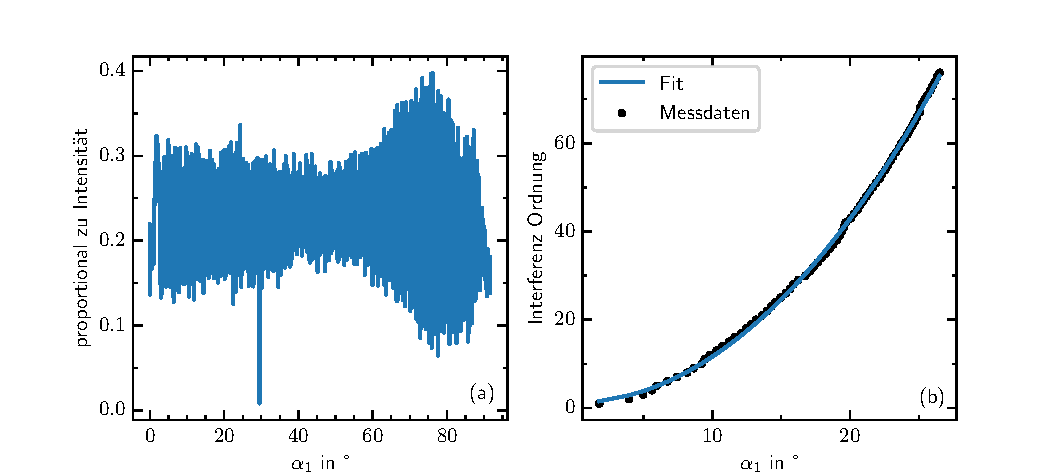
\includegraphics[scale=0.7]{pictures/glas_ausw.pdf}\label{fig:aufbau}
    \caption{\textbf{Interferenz in Abhängigkeit vom Winkel des Glasplättchens.} (a) Der Intensitätsverlauf in Abhängigkeit des Winkels $\alpha_1$ zwischen Laserstrahl und Flächennormale des Plättchens. Die absolute Intensität soll hier nicht betrachtet werden. Deshalb ist die Spannung in V auf der y-Achse nicht in Intensität des Lichts umgerechnet. Es soll nur der qualitative Verlauf gezeigt werden. (b) Die Maxima des oszillierenden Verlaufs aus (a) werden abgezählt und somit einer Ordnungsnummer zugeordnet. Die Ornungsnummer wird dann gegen die Winkelposition des Glasplättchens aufgetragen. Das Erbebnis einer Anpassung an die Daten gemäß [Gleichung zitieren] ist ebenfalls angegeben.}
\end{figure}
Aus \figref{fig:ausw_glas}(a) lässt sich der Intensitätsverlauf des von der Photodiode gemessenen Lichts in Abhängigkeit von $\alpha_1$ ablesen. Die Intensität oszilliert wie erwartet mit dem Winkel des Glasplättchens. Deren Periode ist allerdings so klein im Vergleich zur Winkelachse, dass man sie kaum erkennen kann. Man erkennt allerdings, dass die Amplitude der Oszillationen mit $\alpha_1$ erst ab- und dann zunimmst, bevor sie bei einem Winkel von $90$° gegen 0 geht. Wenn man alle Maxima aus \figref{fig:ausw_glas}(a) identifiziert und durchnummeriert, erhält man  \figref{fig:ausw_glas}(b). Hier Ist die Nummerierungszahl des jedes Maximums gegen den Winkel bei dem es auftritt aufgetragen. Die Ornung der Maxima folgt theoretisch Gleichung soundso. Durch Anpassen der Funktion
\begin{align*}
I_\text{fit}(\alpha_1,n,B,c,d)=2\,\frac{b}{\lambda}\,\left( \sqrt{n^2-\sin^2(\alpha_1-d)}- \cos(\alpha_1-d) \right)-c
\end{align*}
lassen sich der Brechungsindex des Plättchens $n$, sowie das Verhältnis zwischen dessen Dicke $b$ und der Wellenlänge des Lasers $\lambda$ abschätzen, $B=b/\lambda$. Der Brechungsindex von Luft wurde näherungsweise auf 1 gesetzt. Um die totale Ordnung der Interferenzmaxima ignorieren zu können und nur relative Ordnungen zu betrachten, wurder die Verschiebung $c$ eingeführt. Der Parameter $d$ kann wiederum eine Offset im Winkel ausgleichen. Das kann nützlich sein, da der Startpunkt im Winkel manuel auf $0$° gestellt wurde. Die Ergebnisse der Anpassung sind die folgenden.
\begin{table}[H]
    \begin{tabular}{}
    &$n$&$B$&$c$&$d$\\\hline
    Wert& 1.6&  841&  1078& -3e-03\\\hline
    Fehler in $\sigma$&0.5, 406& 441& 1e-02
    \end{tabular}
    \caption{}
\end{table}
Man sieht, dass der Fitwert für den Brechungsindex ungefähr in der richtigen Richtung liegt, jedoch mit sehr großer Unsicherheit. Ähnliches gilt für die Dicke des Plättchens, das mit $0.46\,$mm einen plausiblen Wert hat. 

Wenden wir uns schließlich der Messung des Brechungsindex von Luft zu. Dabei wurde eine Gaszelle der Länge $10\pm0.1\,$cm in einen der Strahlengänge eingebracht.
